% Chapter 6 of Volume III: Bondesson's letter, the gamma block and the levels 3/4 and 7/8. Sources: misc/reviews/nick-volume3/vol3/chG_bondesson.tex lines 3-441; reports U08 (M1 to M9 and minors), V3A rows bo:thm:level and bo:prop:descent; verification W4 (V12). 17 Nov 2026.
\label{bo:ch:bondesson}

% TODO for the authors: the 2016 letter and Abramowitz and Stegun 6.1.50 have no bib entry.
In a letter dated Ume\aa, 23 August 2016, Lennart Bondesson showed that $g(s)=e^{-\gamma\sqrt s}/\Gamma(1+\sqrt s)$ is the Laplace transform of a generalised gamma convolution (GGC), where $\gamma$ is Euler's constant. Since $1-\cos x=2\sin^2(x/2)$, his argument is the gamma function case of the sine squared lemma \eqref{eq:sin2}. This chapter keeps the material of an unrefereed note of Polson (November 2026) written around the letter, with credit and cross references where Volumes I and II already contain a statement. It gives a proof of the sign condition in the letter, which Bondesson had checked with Maple plots, a closed form for the Thorin density, and a generalisation to every centred infinitely divisible law with only negative jumps (Theorem~\ref{bo:thm:gen}).

The level criterion of Section~\ref{bo:sec:level} says that $\xi(\alpha)/\xi(\alpha+\sqrt s)$ is a GGC transform exactly when no zero lies to the right of $\alpha$. It is Theorem~\ref{thm:poisson}, with Proposition~\ref{prop:struct} and Remark~\ref{rem:ch2:oneline}; we give a proof through the Hadamard product, which also covers zeros on the line $\Re s=\alpha$. The Thorin density splits into an archimedean part, which together with the pole term integrates on the critical line to $\theta(T)/\pi$ exactly, and a zeta part that carries $1+S(T)$. The rest of the chapter is computation: the level $\frac34$ with a deconvolution to the critical line, and the level $\frac78$, where the zero free half plane $\Re s>\frac78$ is the theorem of \cite{OAI26a} (Section~\ref{qrh:sec:claims}). A descent criterion (Proposition~\ref{bo:prop:descent}, which is Theorem~\ref{tf:thm:deconv} with a signed variant) turns the deconvolution into an exact test of RH.

For computation in the strip the letter helps: subtracting the archimedean part first lets one linear solve replace the iteration, and improves the counting function by a factor of 9 to 62 on exact data and 1.4 to 4.9 on the data of Section~\ref{bo:sec:speed}. For understanding, it names what has to cancel. For proof inside the strip it adds nothing. Below $\alpha=1$ the L\'evy decomposition of the arithmetic part fails, since its drift is infinite and the truncated drifts grow like a power of the cutoff. Every argument of this kind loses a power of the cutoff against a margin of the size of its logarithm, and positivity there is equivalent to the location of the zeros.

\section{The letter}

Bondesson's letter makes one claim and five remarks:
\begin{description}
\item[(Claim)] The function $g(s)=e^{-\gamma\sqrt s}/\Gamma(1+\sqrt s)$ is the Laplace transform of a GGC, and hence HCM.
\item[(Remark 1)] $\tilde g(s)=e^{-\gamma s}/\Gamma(1+s)$ is not even completely monotone. He adds, with the comment ``I think'', that the same holds for $s^b$ with $b>\frac12$.
\item[(Remark 2)] Since $e^{-c\sqrt s}$ is HCM for $c\ge0$, $g$ may be multiplied by $T^{\sqrt s}$ with $0<T\le1$.
\item[(Remark 3)] $s$ may be replaced by $s^\alpha$ with $0<\alpha\le1$.
\item[(Remark 4)] $\Gamma(1+\sqrt s)$ may be replaced by $\Gamma(a+\sqrt s)$ with $a\ge1$.
\item[(Remark 4$'$)] (The letter has a second Remark 4.) $g$ is not the transform of an HCM density: the Pick test on $g^{(n+1)}/g^{(n)}$ holds for $n=0,1,2$ and fails at $n=3$.
\end{description}
He closes by suggesting the law with transform $\exp\{-(e^{-\sqrt s}-1+\sqrt s)\}$ as worth further study.

\subsection{The exponent}

From Abramowitz and Stegun, formula 6.1.50, and the identity $-\gamma=\int_0^\infty(1-t/(1-e^{-t}))e^{-t}t^{-1}\,dt$, Bondesson writes $g=e^{-h}$ with
\begin{equation}\label{bo:eq:h}
h(s)=\log\Gamma(1+\sqrt s)+\gamma\sqrt s=\int_0^\infty\big(e^{-t\sqrt s}-1+t\sqrt s\big)\frac{e^{-t}}{1-e^{-t}}\frac{dt}{t}.
\end{equation}
To check \eqref{bo:eq:h}, differentiate in $z=\sqrt s$: the right side gives $\int_0^\infty(1-e^{-zt})e^{-t}(1-e^{-t})^{-1}\,dt=\sum_{n\ge1}(1/n-1/(n+z))=\psi(1+z)+\gamma$, the derivative of the left side, and both sides vanish at $z=0$.

\subsection{The Pick reduction}

By the characterisation of GGC transforms in \cite[Chapter 3]{Bondesson}, $g$ is a GGC transform as soon as $-h'(s)$ is a Pick function, that is, holomorphic on $\mathbb C\setminus(-\infty,0]$ with nonnegative imaginary part for $\Im s>0$, and $h'\ge0$ on $(0,\infty)$. % UNVERIFIED: the theorem numbers 3.1.2 and 3.1.3 of Bondesson (1992) were not checked, so only the chapter is cited.
Differentiating \eqref{bo:eq:h},
\[
-h'(s)=\int_0^\infty\frac{e^{-t\sqrt s}-1}{\sqrt s}\,\frac12\,\frac{e^{-t}}{1-e^{-t}}\,dt,
\]
so it is enough that $\Im[(e^{-t\sqrt s}-1)/\sqrt s]\ge0$ when $\Im s>0$. By rescaling one may take $t=1$. With $s=re^{i\theta}$ and $\eta=\theta/2\in(0,\frac\pi2)$, the imaginary part is
\begin{equation}\label{bo:eq:F}
\frac{1}{\sqrt r}\Big(\sin\eta-e^{-\sqrt r\cos\eta}\sin(\eta+\sqrt r\sin\eta)\Big).
\end{equation}
The letter verifies this sign with Maple plots. The next lemma proves it.

\begin{lemma}[Damped sine]\label{bo:lem:ds}
For $\rho>0$, $0\le\eta\le\frac\pi2$ and $w=\rho e^{i\eta}$,
\[
\Im\Big[\frac{e^{-w}-1}{w}\Big]=\frac1\rho\int_0^\rho e^{-v\cos\eta}\sin(v\sin\eta)\,dv\ \ge\ 0.
\]
\end{lemma}

\begin{proof}
Write $(e^{-w}-1)/w=-\int_0^1e^{-uw}\,du$, take imaginary parts, and substitute $v=u\rho$. If $\eta=0$ the integral is $0$. Otherwise the substitution $y=v\sin\eta$ turns it into $(\sin\eta)^{-1}\int_0^{\rho\sin\eta}e^{-y\cot\eta}\sin y\,dy$. Because $\cot\eta\ge0$, the lobes of $e^{-y\cot\eta}\sin y$ on $[k\pi,(k+1)\pi]$ alternate in sign and do not increase in area, so every partial integral is nonnegative.
\end{proof}

Differentiating in $\rho$ gives $\int_0^\rho e^{-v\cos\eta}\sin(v\sin\eta)\,dv=\sin\eta-e^{-\rho\cos\eta}\sin(\eta+\rho\sin\eta)$, which is \eqref{bo:eq:F} with $\rho=\sqrt r$. On the cut, where $\eta=\frac\pi2$, the expression becomes $1-\cos\rho=2\sin^2(\rho/2)$. This is the kernel of the sine squared lemma.

\begin{figure}[ht]
\centering
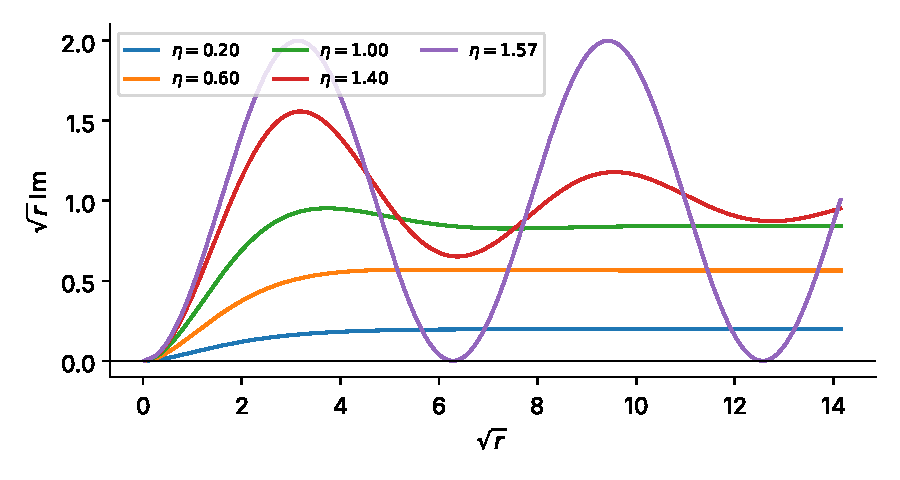
\includegraphics[width=\textwidth]{fig/v3/bo_pick.pdf}
\caption{$\sqrt r$ times the imaginary part \eqref{bo:eq:F}, plotted against $\sqrt r$. The top curve, $\eta=\pi/2$, is $1-\cos\sqrt r$.}
\label{bo:fig:pick}
\end{figure}

\subsection{The Thorin density in closed form}

Stieltjes inversion gives Bondesson's formula for the Thorin density in the variable $r$ (the variable $z$ of the book; the digamma block below is the term $A$ of Remark~\ref{tx2:rem:alpha1}),
\[
u(r)=\frac1\pi\int_0^\infty\frac{1-\cos(t\sqrt r)}{\sqrt r}\,\frac12\,\frac{e^{-t}}{1-e^{-t}}\,dt.
\]
Expanding $e^{-t}/(1-e^{-t})=\sum_{n\ge1}e^{-nt}$ and using $\int_0^\infty(1-\cos bt)e^{-nt}\,dt=b^2/\{n(n^2+b^2)\}$ gives
\begin{equation}\label{bo:eq:u}
u(r)=\frac{\gamma+\Re\,\psi(1+i\sqrt r)}{2\pi\sqrt r}=\frac{1}{2\pi\sqrt r}\sum_{n\ge1}\frac{r}{n(n^2+r)}.
\end{equation}
As $r\to0$, $u(r)\sim\zeta(3)\sqrt r/(2\pi)$. As $r\to\infty$, $u(r)\sim\log r/(4\pi\sqrt r)$. Quadrature of Bondesson's integral and the closed form \eqref{bo:eq:u} agree to fourteen digits at $r=0.1,1,10,100$ (computed; Figure~\ref{bo:fig:u}).

\begin{figure}[ht]
\centering
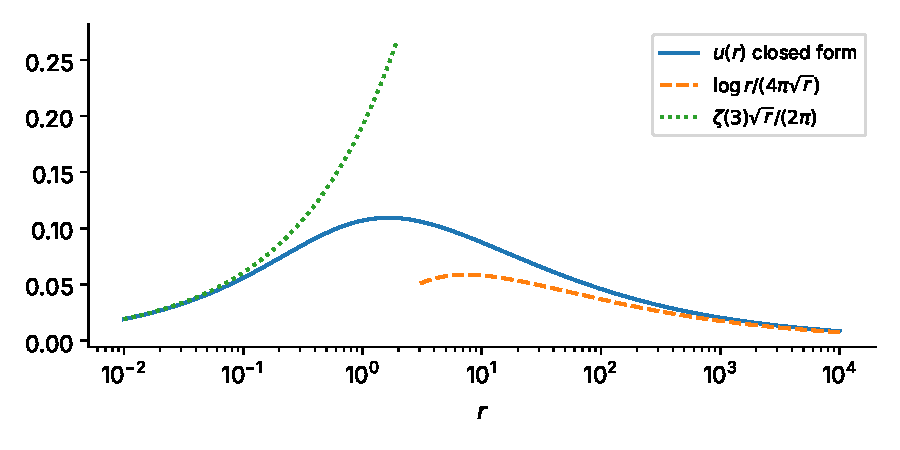
\includegraphics[width=\textwidth]{fig/v3/bo_udens.pdf}
\caption{The Thorin density \eqref{bo:eq:u} with its small and large $r$ asymptotes.}
\label{bo:fig:u}
\end{figure}

\section{The probabilistic content of the letter}

Let $\gamma_a$ be gamma distributed with shape $a$, and put $X_a=\log\gamma_a-\psi(a)$. Since $\E\gamma_a^z=\Gamma(a+z)/\Gamma(a)$,
\begin{equation}\label{bo:eq:ga}
g_a(s):=\frac{\Gamma(a)\,e^{\psi(a)\sqrt s}}{\Gamma(a+\sqrt s)}=\frac{1}{\E e^{\sqrt s\,X_a}},\qquad g_1=g.
\end{equation}
So Bondesson's function is the reciprocal of the moment generating function of a centred log gamma variable at $\sqrt s$. $X_a$ is infinitely divisible with only negative jumps and L\'evy measure $\nu_a(dx)=e^{-ax}\,dx/\{x(1-e^{-x})\}$.

\begin{theorem}\label{bo:thm:gen}
Let $X$ be infinitely divisible with $\E X=0$ and
\[
\log\E e^{zX}=\tfrac12c^2z^2+\int_0^\infty\big(e^{-zx}-1+zx\big)\,\nu(dx),\qquad\Re z\ge0,
\]
where $\int_0^\infty\min(x,x^2)\,\nu(dx)<\infty$. Then $G(s)=1/\E e^{\sqrt sX}$ is the Laplace transform of a GGC with drift $c^2/2$. Its Thorin measure, written in the variable $t=\sqrt r$, is
\begin{equation}\label{bo:eq:Ugen}
U(dt)=\frac1\pi\int_0^\infty\big(1-\cos tx\big)\,x\,\nu(dx)\,dt .
\end{equation}
\end{theorem}

\begin{proof}
Differentiating gives $(\log G)'(s)=-\frac{c^2}{2}+\int_0^\infty x\,\frac{e^{-x\sqrt s}-1}{2\sqrt s}\,\nu(dx)$. For $\Im s>0$ and $x>0$, Lemma~\ref{bo:lem:ds} applied with $w=x\sqrt s$ shows each integrand has nonnegative imaginary part, so $(\log G)'$ is a Pick function, and it is negative on $(0,\infty)$. Bondesson's criterion then makes $G$ a GGC transform. At $s=-t^2+i0$, $\sqrt s=it$, and $\Im[(e^{-ixt}-1)/(2it)]=(1-\cos xt)/(2t)$. With $dr=2t\,dt$, Stieltjes inversion gives \eqref{bo:eq:Ugen}.
\end{proof}

\begin{remark}[Relation to the sine squared lemma]
In the chart $\theta=\sqrt z$ the sine squared lemma \eqref{eq:sin2} reads $e^{-sx}+sx-1=\frac x\pi\int_0^\infty\log(1+s^2/\theta^2)(1-\cos x\theta)\,d\theta$. Integrating it against $\nu(dx)$ gives \eqref{bo:eq:Ugen}, so Theorem~\ref{bo:thm:gen} is the sine squared lemma stated for a L\'evy measure $\nu$. The letter is the case $\nu=\nu_1$.
\end{remark}

\subsection{Remark 4 sharpened}

\begin{proposition}\label{bo:prop:sharp}
For every $a>0$ and $\beta\in\mathbb R$, the function $\Gamma(a)e^{-\beta\sqrt s}/\Gamma(a+\sqrt s)$ is a GGC transform if and only if $\beta\ge-\psi(a)$. Its Thorin density is
\[
u_{a,\beta}(r)=\frac{\Re\,\psi(a+i\sqrt r)-\psi(a)}{2\pi\sqrt r}+\frac{\beta+\psi(a)}{2\pi\sqrt r}.
\]
\end{proposition}

\begin{proof}
The function equals $g_a(s)\,e^{-(\beta+\psi(a))\sqrt s}$. For $c\ge0$ the factor $e^{-c\sqrt s}$ is a GGC transform with Thorin density $c/(2\pi\sqrt r)$ in $r$, because $\sqrt u=\pi^{-1}\int_0^\infty\log(1+u/\theta^2)\,d\theta$ (Remark 2 of the letter). So if $\beta+\psi(a)\ge0$, the function is a product of two GGC transforms, by \eqref{bo:eq:ga} and Theorem~\ref{bo:thm:gen}. If $\beta+\psi(a)<0$, the expansion near $s=0$ is $1-(\beta+\psi(a))\sqrt s+O(s)$, which exceeds $1$ for small $s>0$. A Laplace transform of a probability measure cannot do that.
\end{proof}

Bondesson keeps $\beta=\gamma=-\psi(1)$. Since $\psi$ is increasing, $\gamma\ge-\psi(a)$ is exactly his condition $a\ge1$. Every $a>0$ works once the drift $e^{\psi(a)\sqrt s}$ is matched to $a$.

\subsection{Remark 1 in one line}

The expansion $\log\{e^{-\gamma z}/\Gamma(1+z)\}=-\sum_{k\ge2}(-1)^k\zeta(k)z^k/k$ has no linear term. Put $z=s^b$ with $b>\frac12$. Then $1-\tilde g(s)=O(s^{2b})=o(s)$. If $\tilde g$ were completely monotone with $\tilde g(0)=1$, its law would have mean $0$ and support in $[0,\infty)$, so it would be $\delta_0$. That forces $\tilde g\equiv1$, which is false. This confirms Bondesson's ``I think''. At $b=\frac12$ the linear term survives with coefficient $\pi^2/12$. This is why the book works with $\xi(\alpha+\sqrt s)$ rather than $\xi(\alpha+s)$ (Remark~\ref{tx3:rem:forced}).

\subsection{The closing example}

Take $\nu=\delta_1$. Then $X=1-N$ with $N$ Poisson with mean one, $1/\E e^{\sqrt sX}=\exp\{-(e^{-\sqrt s}-1+\sqrt s)\}$, and \eqref{bo:eq:Ugen} gives $U(dt)=\pi^{-1}(1-\cos t)\,dt$. A single jump of size $x$ produces the periodic Thorin density $\pi^{-1}x(1-\cos tx)$.

\section{The level criterion}\label{bo:sec:level}

For $\alpha\ge\frac12$, put $G_\alpha(s)=\xi(\alpha)/\xi(\alpha+\sqrt s)$, the shifted clock of Section~\ref{ch:clock}. At $s=-t^2+i0$ we have $\sqrt s=it$. The Stieltjes inversion of the proof of Theorem~\ref{bo:thm:gen} gives the formal Thorin density in the variable $t=\sqrt r$, which is the chart $\theta=\sqrt z$ of \eqref{eq:Ualpha}:
\begin{equation}\label{bo:eq:Ualpha}
U_\alpha(dt)=\frac1\pi\,\Re\frac{\xi'}{\xi}(\alpha+it)\,dt=\frac1\pi\,d_t\arg\xi(\alpha+it).
\end{equation}

\begin{theorem}[Level criterion]\label{bo:thm:level}
Let $\alpha\ge\frac12$. Then $G_\alpha$ is the Laplace transform of a GGC if and only if $\xi$ has no zeros in $\Re s>\alpha$. In that case
\[
U_\alpha(dt)=\frac1\pi\sum_\rho\frac{\alpha-\beta}{(\alpha-\beta)^2+(t-\gamma)^2}\,dt\qquad(t>0),
\]
where the sum runs over the zeros $\rho=\beta+i\gamma$ (ordinates of both signs, with multiplicity), and a zero with $\beta=\alpha$ contributes an atom at its ordinate.
\end{theorem}

This is Theorem~\ref{thm:poisson} (after \cite{P26}), and the density formula is Proposition~\ref{prop:struct} at $\alpha=\frac12+\varepsilon$.

\begin{proof}
Suppose $\xi$ has a zero $\rho$ with $\beta>\alpha$. Then $u=(\rho-\alpha)^2$ has $\Re\sqrt u=\beta-\alpha>0$, so it lies in the slit plane $\mathbb C\setminus(-\infty,0]$, and $G_\alpha$ has a pole there, since $\xi(\alpha)\ne0$. A GGC transform is holomorphic and zero free on the slit plane, so $G_\alpha$ is not one.

Conversely, suppose there are no zeros in $\Re s>\alpha$. Put $w=\sqrt u$. By Hadamard's product, grouping each zero $\rho=\beta+i\gamma$ with $\gamma>0$ with its conjugate $\bar\rho$,
\[
\frac{\xi(\alpha+w)}{\xi(\alpha)}=\prod_{\rho}\Big(1-\frac{w}{\rho-\alpha}\Big)=\prod_{\gamma>0}F_\rho(w),\qquad F_\rho(w)=\frac{(c+w)^2+\gamma^2}{c^2+\gamma^2},
\]
where $c=\alpha-\beta\ge0$, and the second product runs over the zeros in the upper half plane, with multiplicity. Indeed $\rho-\alpha=-c+i\gamma$, and $(1+w/(c-i\gamma))(1+w/(c+i\gamma))=F_\rho(w)$. The product converges absolutely, locally uniformly in $w$, since $F_\rho(w)-1=(2cw+w^2)/(c^2+\gamma^2)$ and $\sum|\rho-\alpha|^{-2}<\infty$.

Fix a zero with $c>0$ and write $\lambda=c+i\gamma$. For $\Re w>0$, the function $t\mapsto1/(w-it)$ is bounded and holomorphic in the upper half plane and $1/(w+it)$ in the lower, so the Poisson integral gives, with $P_c(x)=c/\{\pi(c^2+x^2)\}$,
\[
\int_{-\infty}^\infty\frac{P_c(t-\gamma)}{t^2+w^2}\,dt=\frac1{2w}\Big[\frac1{w+\bar\lambda}+\frac1{w+\lambda}\Big]=\frac{(c+w)}{w\{(c+w)^2+\gamma^2\}} .
\]
By the symmetry $t\mapsto-t$ the left side is $\int_0^\infty[P_c(t-\gamma)+P_c(t+\gamma)]\,(t^2+s)^{-1}\,dt$ with $s=w^2$, and the right side is $\frac{d}{ds}\log F_\rho(\sqrt s)$. Both sides vanish at $s=0$ after integrating, so for $s>0$
\[
\log F_\rho(\sqrt s)=\int_0^\infty\log\Big(1+\frac s{t^2}\Big)\big[P_c(t-\gamma)+P_c(t+\gamma)\big]\,dt .
\]
For $c=0$ the factor is $F_\rho=1+s/\gamma^2$, which is the same identity with the kernel replaced by the atom $\delta_\gamma$. Let $U$ be the sum over $\gamma>0$ of these kernels. The terms are positive, so by Tonelli $\int\log(1+s/t^2)\,U(dt)=\sum\log F_\rho(\sqrt s)<\infty$ for $s>0$. Finiteness at $s=1$ is Thorin's integrability condition, so $G_\alpha(u)=\exp\{-\int\log(1+u/t^2)\,U(dt)\}$ is the Laplace transform of a GGC with zero drift. Its Thorin density is the displayed sum, which agrees with \eqref{bo:eq:Ualpha} by Hadamard's formula.
\end{proof}

\begin{corollary}\label{bo:cor:level}
\begin{enumerate}
\item $U_\alpha\ge0$ for every $\alpha\ge1$ unconditionally, because every zero has $\beta<1$.
\item At $\alpha=\frac12$, GGC is equivalent to RH, and then $U_{1/2}=\sum_{\gamma>0}\delta_\gamma$ (with multiplicity) in $t$, which is $\sum_{\gamma>0}\delta_{\gamma^2}$ in the variable $z$.
\item If $\xi$ has no zeros in $\Re s>\theta$, then $U_\alpha$ is a Thorin measure for every $\alpha\ge\theta$. In particular this holds for $\theta=\frac78$ by \cite{OAI26a}.
\item Under RH, $U_\alpha=P_{\alpha-1/2}*U_{1/2}$, where $P_\delta(t)=\delta/\{\pi(\delta^2+t^2)\}$ is the Poisson (Cauchy) kernel and $U_{1/2}$ is extended evenly in $t$.
\end{enumerate}
\end{corollary}

Lagarias \cite{Lagarias,Garunkstis02} proved that RH is equivalent to $\Re\,\xi'/\xi(s)>0$ on $\Re s>\frac12$. Theorem~\ref{bo:thm:level} restates this as a GGC property, one level at a time. Sondow and Dumitrescu \cite{SD10} give the equivalent monotonicity formulation: $|\xi(\sigma+it)|$ is increasing in $\sigma>\frac12$. On a single line the sign of $\Re\,\xi'/\xi$ and the GGC property differ (Remark~\ref{rem:ch2:oneline}).

\section{Archimedean and arithmetic parts}

Write $\xi(s)=(s-1)\pi^{-s/2}\Gamma(1+s/2)\zeta(s)$ and set $a=1+\alpha/2$. Taking real parts of the logarithmic derivative in \eqref{bo:eq:Ualpha} gives, as a regrouping of \eqref{eq:split} for $\alpha>1$,
\begin{equation}\label{bo:eq:split}
\pi\frac{dU_\alpha}{dt}=\underbrace{B_\alpha(t)+c_\alpha}_{\text{archimedean}}+\underbrace{\Pi_\alpha(t)+A_\alpha(t)}_{\text{arithmetic}},
\end{equation}
where
\begin{align*}
B_\alpha(t)&=\tfrac12\big[\Re\,\psi(a+\tfrac{it}2)-\psi(a)\big]\ \ge\ 0,&
c_\alpha&=\tfrac12\big[\psi(a)-\log\pi\big],\\
\Pi_\alpha(t)&=\Re\,(\alpha-1+it)^{-1},&
A_\alpha(t)&=\Re\,\tfrac{\zeta'}{\zeta}(\alpha+it).
\end{align*}
The term $\pi^{-1}B_\alpha$ is the Thorin density, in $t$, of the letter's transform $g_a(s/4)$ (Proposition~\ref{bo:prop:sharp} with the scaling $s\mapsto s/4$). It vanishes like $t^2$ at $0$ and grows like $\frac1{2\pi}\log t$. The constant $c_\alpha$ comes from $\pi^{-s/2}$ and the matched drift. In the strip $\psi(a)\le\psi(\frac32)\approx0.036<\log\pi$, so $c_\alpha<0$. The pole term and the zeta term are grouped because both are singular at $s=1$ and only their sum is harmonic.

\begin{proposition}[Harmonic structure]\label{bo:prop:harm}
The archimedean density $B_\alpha(t)+c_\alpha=\Re\,\frac{d}{ds}\log\{\pi^{-s/2}\Gamma(1+s/2)\}$ at $s=\alpha+it$ is harmonic in $\Re s>-2$ and grows logarithmically. Hence, for $\alpha\ge\alpha_0>-2$, it is the Poisson extension of its values at level $\alpha_0$. The arithmetic density $\Pi_\alpha+A_\alpha=\Re\,\frac{d}{ds}\log\{(s-1)\zeta(s)\}$ is harmonic away from the zeros of $\zeta$. In particular it is harmonic in $\Re s>\frac12$ under RH.
\end{proposition}

\subsection{The critical line: the letter gives $\theta(T)/\pi$}

At $\alpha=\frac12$ we have $a=\frac54$. Integrate the archimedean part and the pole term over $[0,T]$, and use $\arg\Gamma(\frac54+\frac{iT}2)=\arg\Gamma(\frac14+\frac{iT}2)+\arctan2T$ and $\arg(-\frac12+iT)-\pi=-\arctan2T$. This gives
\[
\frac1\pi\Big[\arg\Gamma(\tfrac54+\tfrac{iT}2)-\tfrac T2\log\pi\Big]+\frac{\arg(-\frac12+iT)-\pi}{\pi}=\frac{\theta(T)}{\pi},
\]
the Riemann Siegel theta function, exactly. The zeta term therefore carries $1+S(T)$, which is the Riemann von Mangoldt formula $N(T)=\theta(T)/\pi+1+S(T)$ (Section~\ref{ch:turing}) read as a split of the Thorin measure (Figure~\ref{bo:fig:cumul}).

\begin{figure}[ht]
\centering
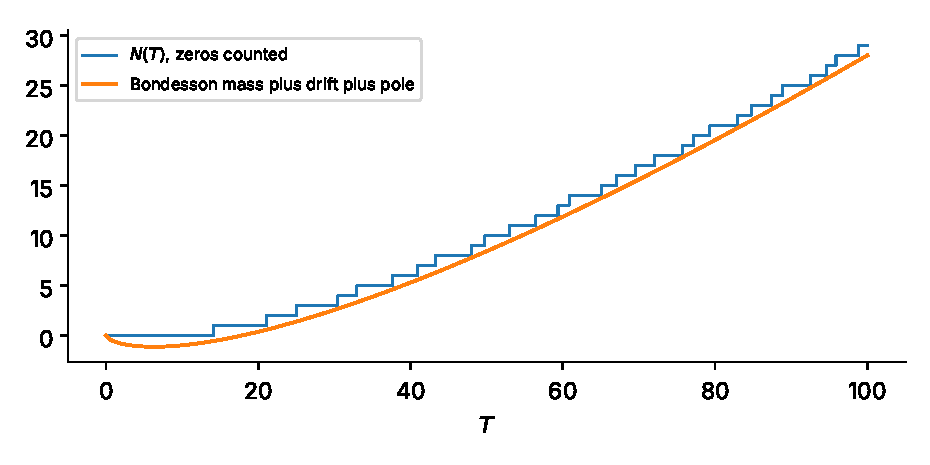
\includegraphics[width=\textwidth]{fig/v3/bo_cumul.pdf}
\caption{$N(T)$ against the integrated archimedean part plus pole term at $\alpha=\frac12$, which equals $\theta(T)/\pi$.}
\label{bo:fig:cumul}
\end{figure}

\subsection{Above the strip}\label{bo:sec:above}

For $\alpha>1$ the split \eqref{eq:split} of Section~\ref{sec:ch6:split} and Proposition~\ref{tx:prop:alpha0} give the following statements; the letter enters in the following form. For $\alpha>1$, $\zeta(\alpha+z)/\zeta(\alpha)=\E e^{-z\log N}$, where $N$ has the zeta distribution $\Pr(N=n)=n^{-\alpha}/\zeta(\alpha)$. This law is infinitely divisible, with L\'evy measure $\sum_n\Lambda(n)(n^\alpha\log n)^{-1}\delta_{\log n}$. Centring it and applying Theorem~\ref{bo:thm:gen} gives the arithmetic Thorin density
\[
\frac1\pi\sum_{n\ge2}\Lambda(n)n^{-\alpha}\big(1-\cos(t\log n)\big)-\frac{\mu_\alpha}{\pi},\qquad \mu_\alpha=-\frac{\zeta'}{\zeta}(\alpha).
\]
Since $\mu_\alpha=\sum\Lambda(n)n^{-\alpha}$, this equals $\pi^{-1}A_\alpha(t)$. The positive sum is the Thorin density of the centred variable and $-\mu_\alpha/\pi$ is its drift. The factor $1/(\alpha-1+\sqrt s)$ is a GGC transform with density $\pi^{-1}(\alpha-1)/\{(\alpha-1)^2+t^2\}$ (the identity for $\log(1+\sqrt u/a)$ in the proof of Proposition~\ref{tx:prop:alpha0}). So for $\alpha>1$ each factor is of Bondesson type, apart from one total drift, the exponential factor $e^{\kappa_\alpha\sqrt s}$ with
\begin{multline*}
\kappa_\alpha=\tfrac12\big(\log\pi-\psi(a)\big)-\frac{\zeta'}{\zeta}(\alpha),\\ \text{positive for }1<\alpha<\alpha_0=5.4962\ldots\ \text{(Proposition~\ref{tx:prop:alpha0})}.
\end{multline*}
For $1<\alpha<\alpha_0$ the drift $\kappa_\alpha>0$ is not a GGC factor and the pole has to pay for it. For $\alpha\ge\alpha_0$, $\kappa_\alpha\le0$, the factor $e^{-|\kappa_\alpha|\sqrt s}$ is itself a GGC factor, and Proposition~\ref{tx:prop:alpha0} gives the Thorin property from the sine squared lemma alone. At $t=0$ only the pole pays: $\frac1{\alpha-1}-\kappa_\alpha=\xi'(\alpha)/\xi(\alpha)>0$.

Below $\alpha=1$ this mechanism breaks for three reasons. The drift $-\zeta'/\zeta(\alpha)\sim1/(\alpha-1)$ blows up. Truncated Euler products are infinitely divisible at every $\alpha>0$, but their drift $\mu_P(\alpha)=\sum_{p\le P}\log p\,p^{-\alpha}/(1-p^{-\alpha})$ grows like $P^{1-\alpha}$. At $P=10^6$ it equals $13.2$ at $\alpha=1$ and $626$ at $\alpha=0.6$ (computed; Figure~\ref{bo:fig:drift}), while the archimedean density grows only like $\frac{1}{2\pi}\log t$. Finally, $\xi(\frac12+z)/\xi(\frac12)=\E e^{zX}$ with $X$ drawn from the Riemann density. Because $\Xi$ has real zeros, $\E e^{i\theta X}=\Xi(\theta)/\Xi(0)$ vanishes on the real line, while the characteristic function of an infinitely divisible law has no real zeros. So $X$ is not infinitely divisible, and Theorem~\ref{bo:thm:gen} does not apply.

\begin{figure}[ht]
\centering
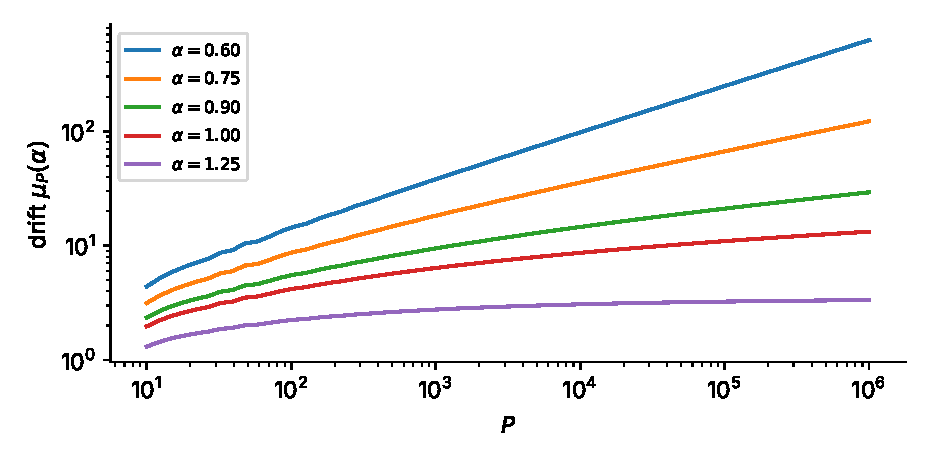
\includegraphics[width=\textwidth]{fig/v3/bo_drift.pdf}
\caption{Drift $\mu_P(\alpha)$ of truncated Euler products, for $P$ up to $10^6$.}
\label{bo:fig:drift}
\end{figure}

\section{The level three quarters}

Throughout this section $\alpha=\frac34$ and $\delta=\frac14$. All numbers are computed in floating point, not certified, from the first 400 zeros (up to $\gamma_{400}=679.74\ldots$) by direct evaluation of \eqref{bo:eq:Ualpha} in 20 digit arithmetic on the grid $t\in[0,130]$ with step $0.05$. Figure~\ref{bo:fig:decomp} shows the split \eqref{bo:eq:split}.

\begin{figure}[ht]
\centering
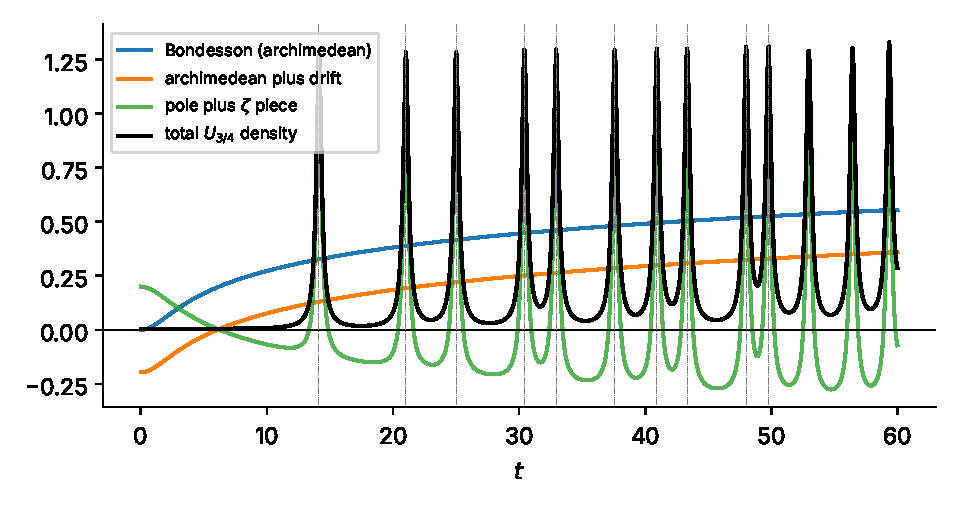
\includegraphics[width=\textwidth]{fig/v3/bo_decomp.pdf}
\caption{The split \eqref{bo:eq:split} at $\alpha=\frac34$, divided by $\pi$. Dotted lines mark the zero ordinates. In this figure the pole term is drawn with the zeta term.}
\label{bo:fig:decomp}
\end{figure}

\subsection{Resolution scales}

The Fourier transform of $P_\delta$ is $e^{-\delta|\omega|}$. Resolving features of size $g$ requires frequencies up to about $\pi/g$, so deconvolution amplifies noise by about $e^{\pi\delta/g}$. At the mean spacing $g=2\pi/\log(T/2\pi)$ this is
\[
e^{\pi\delta/g}=\Big(\frac{T}{2\pi}\Big)^{\delta/2},
\]
which is only polynomial in $T$. Peaks remain separate while the mean spacing exceeds $2\delta$, that is, up to $T=2\pi e^{\pi/\delta}$ (Table~\ref{bo:tab:res}). For $\delta=\frac14$, peaks separate up to $T\approx1.8\times10^6$. Close pairs are the hard cases: a gap $g$ costs $e^{\pi\delta/g}$, so a Lehmer pair with $g=0.04$ needs about nine digits at level $\frac34$.

\begin{table}[ht]
\centering
\begin{tabular}{lcccccc}
\toprule
$T$ & $10^2$ & $10^3$ & $10^4$ & $10^6$ & $10^9$ & $10^{12}$\\
\midrule
mean spacing & 2.27 & 1.24 & 0.85 & 0.52 & 0.33 & 0.24\\
$(T/2\pi)^{1/8}$ & 1.41 & 1.88 & 2.51 & 4.47 & 10.6 & 25.1\\
$(T/2\pi)^{3/16}$ & 1.68 & 2.59 & 3.98 & 9.45 & 34.5 & 126\\
\bottomrule
\end{tabular}
\caption{Mean zero spacing and noise amplification at the mean spacing, for the levels $\frac34$ ($\delta=\frac14$, middle row) and $\frac78$ ($\delta=\frac38$, bottom row).}
\label{bo:tab:res}
\end{table}

\subsection{Deconvolution to the critical line}

Two deconvolution experiments, computed in floating point and not certified, recover the zeros from the data at level $\frac34$: positivity constrained EM finds all 29 zeros below $100$ with location errors at most $0.0021$, and Tikhonov filtering of the arithmetic remainder, with the archimedean part added back exactly, improves the counting function error by a factor of 9 to 62 on exact data but only 1.4 to 4.9 on the data of Section~\ref{bo:sec:speed}.

\subsection{Does the closed form speed up the descent?}\label{bo:sec:speed}

The archimedean part is known exactly at every level and moves between levels by the Poisson semigroup (Proposition~\ref{bo:prop:harm}). Does this make the deconvolution faster, and not only more accurate? We tested four ways of using it, on the descent from $\frac34$ to $\frac12$ on $[0,130]$ with step $0.05$, with the density built from the zeros below height $7000$ and a smooth tail (computed).

% UNVERIFIED: EM and Tikhonov deconvolution not recomputed (W4 NOT DONE).
\begin{enumerate}
\item EM started from the archimedean density at level $\frac12$, which is $\theta'(t)/\pi+2/\{\pi(1+4t^2)\}$, in place of a flat start. The largest location error and the misfit are the same as from the flat start, to the digits printed: $0.0026$ and $0.237$ after $25$ iterations, $0.0021$ and $0.022$ after $3000$. All $29$ zeros are found after $25$ iterations either way.
\item EM with the data corrected for everything above the window, which the harmonic structure gives in closed form. The location errors are unchanged and the misfit is slightly worse.
\item Conjugate gradient iterations on the normal equations, for the raw density and for the arithmetic remainder. The count error at midpoints stalls at $0.08$ for the raw density (after $17$ iterations) and $0.10$ for the remainder.
\item One linear solve by FFT with Tikhonov filtering. It takes $0.9$ milliseconds. With the archimedean part removed first, the count error at midpoints is $0.008$, against $0.011$ to $0.039$ for the raw density, and the zeros are located to $0.0003$ at $\lambda=10^{-3}$ in both cases. EM takes $0.1$ seconds for $25$ iterations and $11.5$ seconds for $3000$, with count error $0.094$ throughout.
\end{enumerate}

The closed form does not reduce the number of iterations of any iterative scheme we tried. EM finds the zeros in about $25$ iterations whatever the start, and the later sharpening of the atoms is governed by the kernel, not the trend. The amplification $e^{\pi\delta/g}$ of Table~\ref{bo:tab:res} belongs to the Poisson kernel, and the gamma factor does not change it.

What the closed form changes is which method can be used. The raw density grows like $\frac1{2\pi}\log t$ and does not extend periodically, so a Fourier method applied to it carries an error from the trend and the edge. With the archimedean part subtracted the remainder has mean zero and a single linear solve is accurate: it is a hundred times faster than the $25$ iterations of EM that find the zeros, locates them more precisely, and gives the counting function ten times more accurately. The letter turns the descent into a problem that one filter solves. EM remains the tool when positivity itself is the question, as in the test with a planted pair, because the linear solve does not know that the answer should be a positive measure.
% UNVERIFIED: EM and Tikhonov deconvolution not recomputed (W4 NOT DONE).

\section{The level seven eighths}

By the theorem of \cite{OAI26a} (Section~\ref{qrh:sec:claims}), $\xi$ has no zeros in $\Re s>\frac78$. By Theorem~\ref{bo:thm:level}, $U_\alpha$ is then a Thorin measure for every $\alpha\ge\frac78$. Here $\delta=\frac38$ and $a=\frac{23}{16}$. The numerical parts compute $U_{7/8}$ from the zeros, wherever they lie.

\subsection{What the letter adds at seven eighths}

The letter does not strengthen the zero free half plane: positivity at $\frac78$ comes from \cite{OAI26a}, and the arithmetic part changes sign, as at $\frac34$. The letter provides:
\begin{enumerate}
\item An explicit archimedean part, $B_{7/8}(t)+c_{7/8}$, with $c_{7/8}/\pi=-0.18595$. The density at $t=0$ is $0.00551$, the global minimum on $[0,130]$, so the arithmetic part must supply $0.19146$ there, a cancellation to three percent. This is an unconditional computation: $\xi(\frac12+x)$ increases with $x$, and the half plane plays no role.
\item Exact detrending (Proposition~\ref{bo:prop:harm}): only the arithmetic remainder has to be deconvolved.
\item A criterion that turns descent into a test of RH, stated next.
\end{enumerate}

\begin{proposition}[Descent from a zero free level]\label{bo:prop:descent}
Suppose $\xi$ has no zeros in $\Re s>\theta$, where $\frac12<\theta\le1$ (for $\theta=1$ this holds unconditionally), and let $\alpha\ge\theta$ with $\alpha>\frac12$. Then RH holds if and only if $U_\alpha=P_{\alpha-1/2}*V$ for some locally finite signed measure $V$ on $\mathbb R$ with $\int(1+t^2)^{-1}|V|(dt)<\infty$. In that case $V=U_{1/2}=\sum\delta_\gamma$ (ordinates of both signs, with multiplicity) and $V\ge0$.
\end{proposition}

For $V\ge0$ this is Theorem~\ref{tf:thm:deconv}, which needs only $\varepsilon_0>\beta-\frac12$ for every zero, for instance $\varepsilon_0\ge\frac12$. Here $V$ may be signed, with positivity as a conclusion, and $U_\alpha$ is extended evenly in $t$ and carries its atoms if a zero lies on $\Re s=\alpha$; then $P_{\alpha-1/2}*V$ is a smooth function, and the equality fails.

The same proof descends from $\alpha$ to any level $\alpha'$ with $\frac12\le\alpha'<\alpha$: there is a locally finite signed measure $V'$ with $\int(1+t^2)^{-1}|V'|(dt)<\infty$ and $U_\alpha=P_{\alpha-\alpha'}*V'$ if and only if $\xi$ has no zeros in $\Re s>\alpha'$, and then $V'=U_{\alpha'}$, with its atoms. This is from an unrefereed note of Polson, November 2026.

\begin{proof}
If RH holds, take $V=U_{1/2}$ and use Corollary~\ref{bo:cor:level}(4). Conversely, suppose such a $V$ exists and put $H(\frac12+y+it)=(P_y*V)(t)$ for $y>0$, which is harmonic in $\Re s>\frac12$. By the semigroup property of the Poisson kernel, on $\Re s>\alpha$ the function $H$ is the Poisson extension of $P_{\alpha-1/2}*V=U_\alpha$. The function $\pi^{-1}\Re\,\xi'/\xi$ is also the Poisson extension of $U_\alpha$ on $\Re s>\alpha$, because every kernel in Proposition~\ref{prop:struct} is positive for $\alpha\ge\theta$ and the Cauchy kernels form a semigroup. So the two agree on $\Re s>\alpha$. The set $\{\Re s>\frac12\}$ minus the zeros of $\xi$ is connected and both functions are real analytic on it, so they agree there. If RH fails, some zero $\rho^*$ has $\Re\rho^*>\frac12$. Letting $s\to\rho^*$ from the right, $\Re\,\xi'/\xi(s)\sim m\Re(s-\rho^*)^{-1}$ is unbounded, where $m$ is the multiplicity, while $H$ is harmonic near $\rho^*$ and hence bounded. This is a contradiction, so RH holds. By Poisson uniqueness, $V$ is then $U_{1/2}$.
\end{proof}

By \cite{OAI26a} and Theorem~\ref{bo:thm:level}, $U_{7/8}=\pi^{-1}\sum_\rho(\frac78-\beta)/\{(\frac78-\beta)^2+(t-\gamma)^2\}$. This is a mixture of Cauchy kernels whose widths $\frac78-\beta$ lie between $0$ and $\frac34$. RH says every width equals $\frac38$. An off line pair $\frac12\pm\varepsilon+i\gamma$ contributes widths $\frac38-\varepsilon$ and $\frac38+\varepsilon$. The wider one deconvolves to a Cauchy kernel of width $\varepsilon$ at level $\frac12$. The narrower one cannot be deconvolved by $P_{3/8}$, and a positivity constrained fit leaves a residual misfit there.


\subsection{Numerics at seven eighths}

At this level the peaks have height between $0.857$ and $0.975$, against $1/(\pi\delta)=0.849$. All 29 zeros below $100$ are still visible separately, and the archimedean part dominates more visibly (Figure~\ref{bo:fig:u78}). EM descent from $\frac78$ to $\frac12$ with 4000 iterations recovers all 29 zeros. The largest location error is $0.0019$, the masses lie between $0.962$ and $0.993$, and the largest relative misfit is $1.4$ percent (computed). Tikhonov descent gives the counting function errors in Table~\ref{bo:tab:tik78}. Here detrending improves accuracy by a factor of 23 to 104 on exact data. Peaks at $\frac78$ separate up to $T=2\pi e^{8\pi/3}\approx2.7\times10^4$ (Table~\ref{bo:tab:res}).
% UNVERIFIED: EM and Tikhonov deconvolution not recomputed (W4 NOT DONE).

\begin{figure}[ht]
\centering
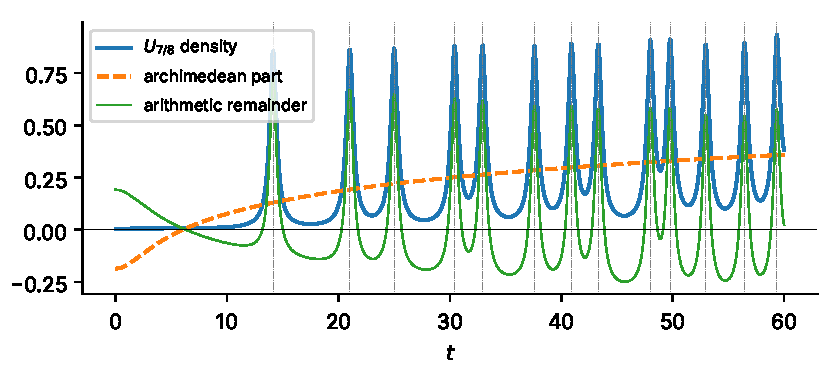
\includegraphics[width=\textwidth]{fig/v3/bo_u78_decomp.pdf}
\caption{$U_{7/8}$, its archimedean part and its arithmetic remainder.}
\label{bo:fig:u78}
\end{figure}

\begin{table}[ht]
\centering
\begin{tabular}{lccc}
\toprule
& $\lambda=10^{-3}$ & $\lambda=10^{-4}$ & $\lambda=10^{-5}$\\
\midrule
raw $U_{7/8}$ & 0.0303 & 0.0555 & 0.0580\\
detrended & 0.0013 & 0.00073 & 0.00056\\
\bottomrule
\end{tabular}
\caption{Largest counting function error at midpoints, after Tikhonov deconvolution from level $\frac78$ (computed, exact data).}
\label{bo:tab:tik78}
\end{table}
% UNVERIFIED: EM and Tikhonov deconvolution not recomputed (W4 NOT DONE).

\subsection{A planted off line pair}

To test Proposition~\ref{bo:prop:descent} in practice, we built $U_{7/8}$ from the Poisson sum over the first 400 zeros. We then moved the tenth zero, $\gamma_{10}=49.774$, to the pair $\frac12\pm\varepsilon+i\gamma_{10}$ and ran EM with the RH width $\frac38$. Table~\ref{bo:tab:pair} reports the largest relative misfit within $3$ of $\gamma_{10}$ and elsewhere below $100$. The misfit floor, set by the grid and the iteration count, is $1.43$ percent. The pair stands out at $\varepsilon=0.05$ (misfit $2.6$ percent) and clearly at $\varepsilon=0.1$ ($6.9$ percent), where the EM estimate splits the atom into two lumps (Figure~\ref{bo:fig:pair}). The experiment is not a detection threshold: the detection size depends on the grid, the iteration count and the tail treatment, and is limited by the amplification $e^{\pi\delta/g}$. A planted pair EM test at level $0.6$ is in Section~\ref{cx:sec:irls}.
% UNVERIFIED: EM and Tikhonov deconvolution not recomputed (W4 NOT DONE).

\begin{table}[ht]
\centering
\begin{tabular}{lccccc}
\toprule
$\varepsilon$ & 0 & 0.02 & 0.05 & 0.1 & 0.2\\
\midrule
misfit near $\gamma_{10}$ (\%) & 1.45 & 1.62 & 2.62 & 6.89 & 26.2\\
misfit elsewhere (\%) & 1.43 & 1.43 & 1.43 & 1.46 & 1.74\\
\bottomrule
\end{tabular}
\caption{EM descent from $\frac78$ with a planted off line pair at height $\gamma_{10}$ (computed).}
\label{bo:tab:pair}
\end{table}
% UNVERIFIED: EM and Tikhonov deconvolution not recomputed (W4 NOT DONE).

\begin{figure}[ht]
\centering
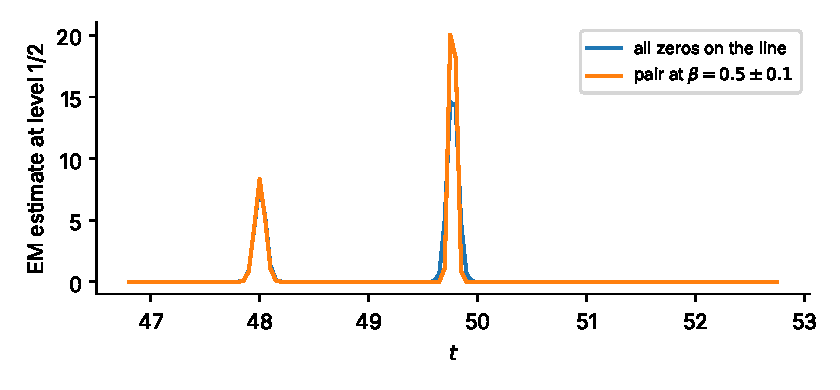
\includegraphics[width=\textwidth]{fig/v3/bo_u78_pair.pdf}
\caption{EM estimate of the measure at level $\frac12$ near $\gamma_{10}$, with all zeros on the line and with a pair at $\beta=\frac12\pm0.1$.}
\label{bo:fig:pair}
\end{figure}
